%==============================================================================
%== template for LATEX poster =================================================
%==============================================================================
%
%--A0 beamer slide-------------------------------------------------------------
\documentclass[final]{beamer}
\usepackage[orientation=portrait,size=a0,
            scale=1.25         % font scale factor
           ]{beamerposter}

\geometry{
  hmargin=2.5cm, % little modification of margins
}

%
\usepackage[utf8]{inputenc}
% diminuir o tamanho da legenda das imagens
\usepackage[font=small,labelfont=bf]{caption}

% pacotes para fluxograma
\usepackage{tikz}
\usetikzlibrary{shapes,arrows}

\renewcommand{\figurename}{Figura}

\linespread{1.15}
%
%==The poster style============================================================
\usetheme{sharelatex}

%==Title, date and authors of the poster=======================================
\title
[24$^{o}$ Simpósio Internacional de Iniciação Científica da USP] % Conference
{ % Poster title
Análise da Dispersão de Material Radioativo por Modelagem Numérica na Baía de Ilha Grande - RJ
}

\author{ Silva, Danilo A.\inst{1} $\&$ Dottori, Marcelo\inst{2}
}
\institute[Instituto Oceanográfico - Universidade de São Paulo]
{
Instituto Oceanográfico da Universidade de São Paulo (IOUSP)\\ [0.2ex]
\inst{1} danilo2.silva@usp.br; \inst{2} mdottori@usp.br
}
\date{\today}



\begin{document}

\begin{frame}
%==============================================================================
\begin{multicols}{2}
%==============================================================================
%==The poster content==========================================================
%==============================================================================

\section{Introdução}

Em escala global, grandes reservatórios d'água são utilizados para despejo de materiais,
sendo que o maior impacto é em regiões de baixa circulação e troca d'água. Grande
parte das usinas nucleares estão instaladas próximas a estes reservatórios, utilizando
suas águas no sistema de resfriamento dos reatores nucleares. No Brasil, existem
duas usinas em funcionamento na Central Nuclear Almirante Álvaro Alberto (CNAAA),
que captam águas e despejam águas na Baía da Ilha Grande (Figura~\ref{fig:areaestudo}),
região de importância turística e sócio ambiental.

Assim, compreender o padrão de circulação da região e avaliar o destino de possíveis
contaminantes radioativos é essencial, no sentido de apoiar os órgãos tomadores de decisão na
eventualidade de tais cenários.

%Usinas nucleares estão instaladas próximas a grandes reservatórios de água,
%utilizando essas águas para resfriar seus reatores, despejando-as em seguida
%no mesmo reservatório, com temperatura e concentração de radioativos alteradas.
%Caso haja algum vazamento no sistema de resfriamento, uma grande quantidade de
%material radioativo poderá ser lançada no ambiente marinho. Atualmente, no Brasil,
%existem duas usinas em operação na Central Nuclear Almirante Álvaro Alberto (CNAAA),
%que captam e despejam águas na Baía da Ilha Grande (Figura~\ref{fig:areaestudo}),
%região de importância turística e sócio ambiental.

\vspace{.1in}
\begin{figure}
\centering
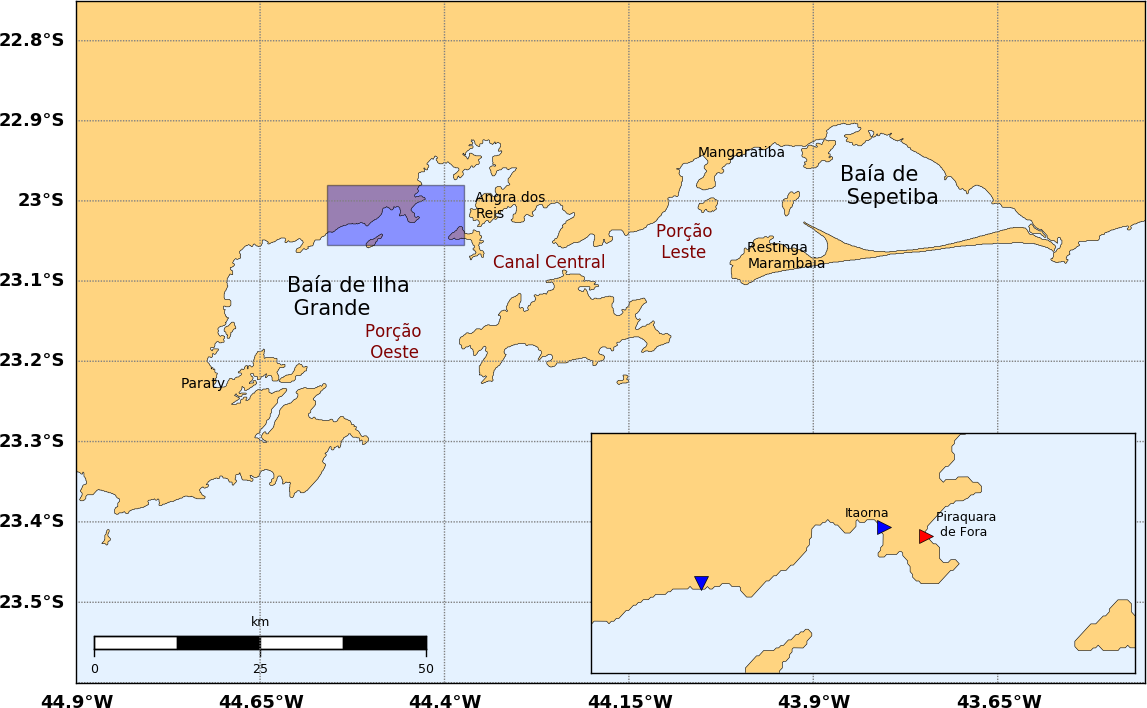
\includegraphics[width=0.8\columnwidth]{/home/tparente/danilo/mestrado/github/congressos/omarsat_2017/poster/sharelatex/figs/imagens_TG/areaestudo2.png}
\vspace{.1in}
\caption{Área de estudo com região de influência direta da CNAAA destacada e ampliada, apresentando a região de obtenção e despejo de água para resfriamento, bem como a classificação fisiográfica.}
\label{fig:areaestudo}
\end{figure}
% \vskip1ex
\vspace{-.5in}

\subsection{Objetivos}

O objetivo deste trabalho é determinar quão impactante seria um cenário de vazamento
nuclear da Central Nuclear. Desta forma, foi analisado como as forçantes vento e maré
influenciam a circulação na região e, então, analisou-se a pluma de dispersão do
material radioativo em diversos cenários típicos da região de estudo.

% ===================================================================================================================
\section{Métodos}

% Para determinar como o vento e a maré,
% principais forçantes, atuam na região, utilizou-
% se o \textit{Stevens Estuarine and Coastal
% Ocean Model}, ou sECOM.
% O modelo possui diversos módulos,
% onde ó módulo hidrodinâmico foi o utilizado
% para modelar a influência de cada variável
% na circulação da região.

\vskip1ex
\begin{figure}
\centering
\includegraphics[width=0.69\columnwidth]{/home/tparente/danilo/mestrado/github/congressos/omarsat_2017/poster/sharelatex/figs/diagramaTGFINAL1.png}
\vspace{.2in}
\caption{Fluxograma da metodologia utilizada no trabalho, onde as caixas vermelhas representam os dados de entrada do modelo, as caixas pretas os módulos do sECOM utilizados e as caixas azuis representam os cenários elaborados, onde de 1 a 4 foram realizados para analisar a influência das forçantes individualmente e de 5 a 7 para analisar a pluma de dispersão do material radioativo.}
\label{fig:metodologia}
\end{figure}
\vskip1ex

% O cenário 3, em vermelho na Fig.~\ref{fig:metodologia}, é o atual estado do trabalho.
% Em seguida o modelo será validado com dado \textit{in situ} e, então, o módulo \textit{Tracer}
% será implementado, a fim de determinar a dispersão do material radioativo despejado.
% \vskip2ex

\vspace{-.7in}
% ===================================================================================================================

\section{Resultados}

Nota-se que os ventos de SW (Figura~\ref{fig:cenariosCirc}.b) apresenta correntes
médias mais intensas quando comparadas ao cenário com ventos de NE
(Figura~\ref{fig:cenariosCirc}.a), onde a geometria da área estudada
favorece ventos de SW com uma maior superfície de contato. Este resultado é
também obtido por [1], onde o transporte gerado por ventos do
quadrante Sul foram maiores que o transporte por ventos do quadrante Norte.
Entretando, ao observamos o cenário somente com maré (Figura~\ref{fig:cenariosCirc}.c),
nota-se que esta forçante gera correntes 2 vezes mais intensas a leste do domínio.

% \vskip.5ex
\begin{figure}
\centering
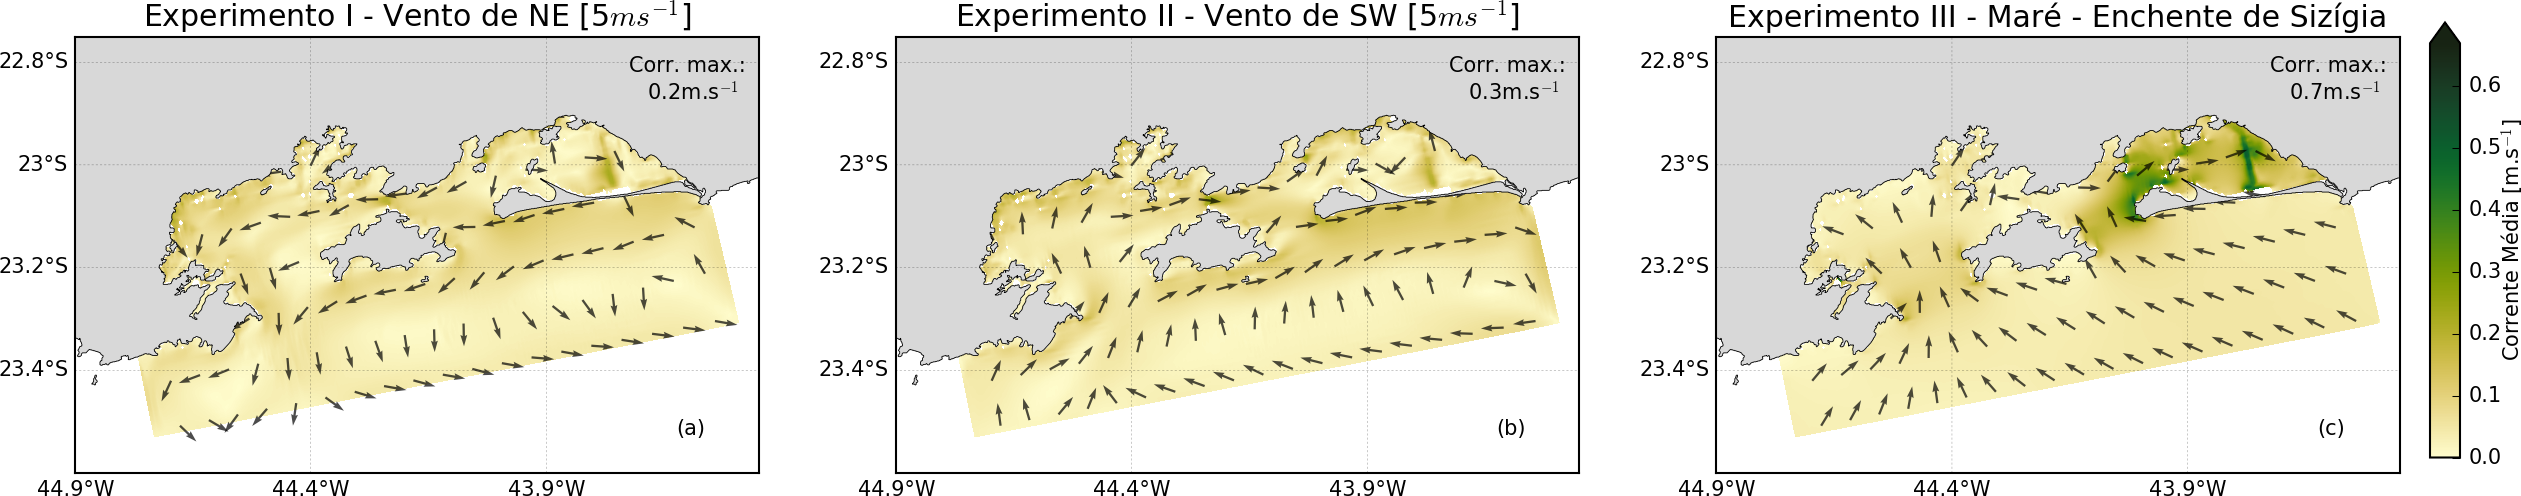
\includegraphics[width=1.\columnwidth]{/home/tparente/danilo/mestrado/github/congressos/omarsat_2017/poster/sharelatex/figs/figura1.png}
\caption{Corrente média nos cenários 1,2 e 3. Os painéis (a) e (b) representam o último instante modelado e (c), o instante da segunda
maré enchente de sizígia do período modelado.}
\label{fig:cenariosCirc}
\end{figure}

\vspace{-1ex}

Comparando os experimentos 5 e 6, notamos que a maior diferença está na direção
preferencial de evolução da pluma, que é comandada pela direção dos ventos em cada
experimento. Entretanto, no experimento 5, os ventos de SW transportam o material
radioativo para leste do domínio, atingindo regiões com correntes mais intensas devido à
influência da maré e, desta forma, diluindo de maneira mais eficaz os radionuclídeos, em
comparação ao experimento 6 que, para o mesmo instante de tempo, possui uma maior
concentração do material na região oeste do domínio (Figura~\ref{fig:cenariosDispersao}).

\vskip1ex
\begin{figure}
\centering
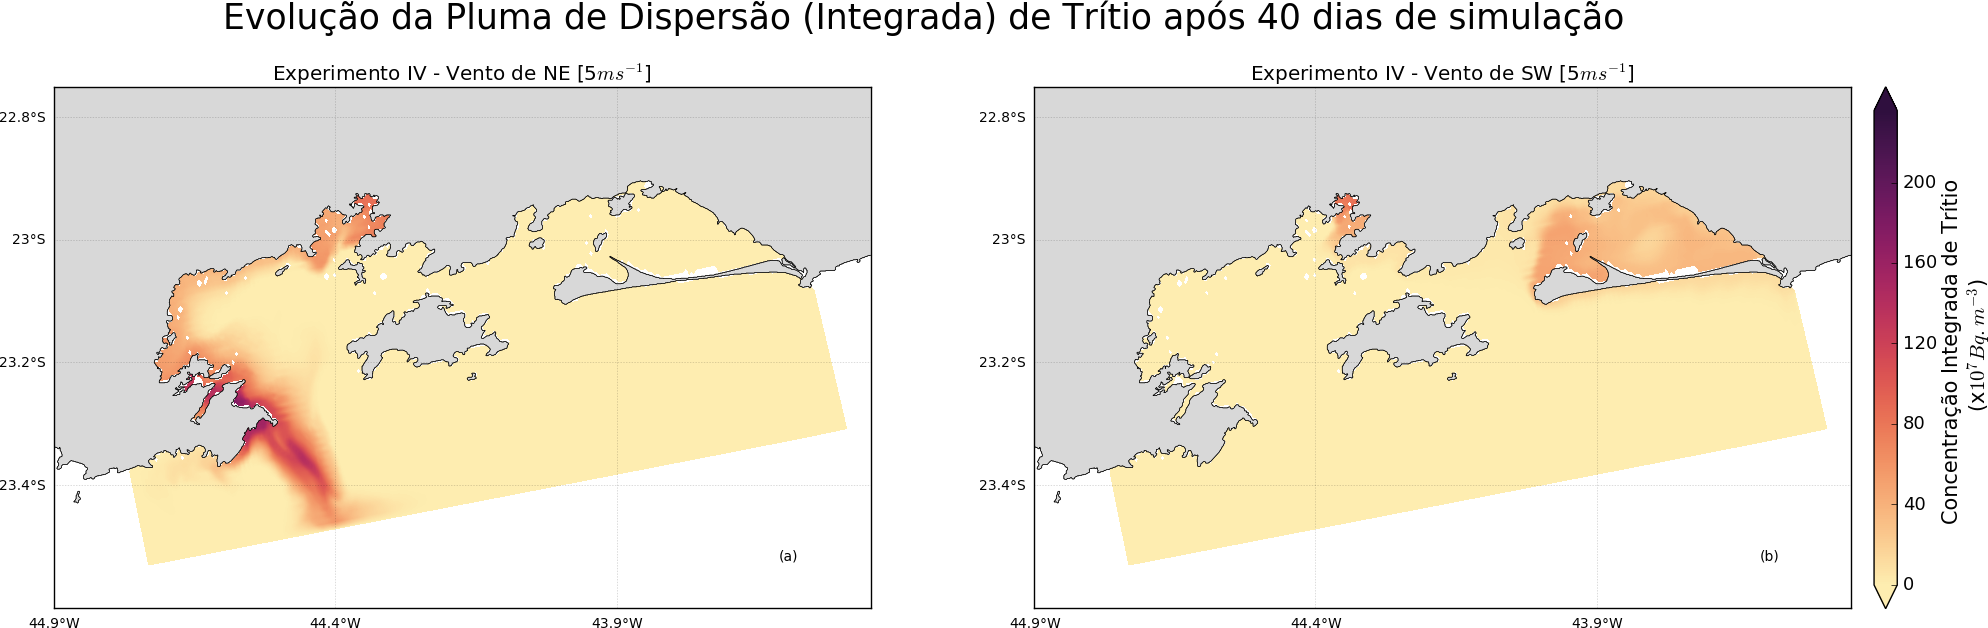
\includegraphics[width=0.99\columnwidth]{/home/tparente/danilo/mestrado/github/congressos/omarsat_2017/poster/sharelatex/figs/figura2_integrada.png}
\caption{Comparação entre os cenários 5 e 6, respectivamente, no instante correspondente a 40 dias de simulação, sendo
a concentração total na coluna.}
\label{fig:cenariosDispersao}
\end{figure}

\vspace{-1ex}

Quanto ao cenário 7 (Figura~\ref{fig:evolucaopluma}), observou-se que a evolução da pluma ocorre,
preferencialmente, para leste do domínio, conforme no cenário 5, onde parte dela
permanece por mais de 30 dias na Baía da Ribeira e outra parte é transportadapara regiões de
correntes mais intensas, sendo rapidamente diluídas. Baseando-se nos cenários 5,6 e 7,
estima-se que levaria mais de 60 dias para que grande parte do material fosse diluído na
região, o que poderia acarretar em sérios problemas para a biota local, onde o material nuclear
seria bio incorporado nos organismos e no sedimento, passando a fazer parte da cadeia alimentar.

%O tempo de permanência é melhor apresentado através da . Notamos
%que, de aproximadamente 150 horas a 500 horas, há uma grande concentração de material nuclear
%na Baía da Ribeira, região de descarte da Central Nuclear. A pluma alcança a região de
%Angra dos Reis a partir das 150 horas simuladas, permanecendo nessa região com uma
%concentração aproximadamente constante até o final da simulação.

\vskip-.4ex
\begin{figure}
\centering
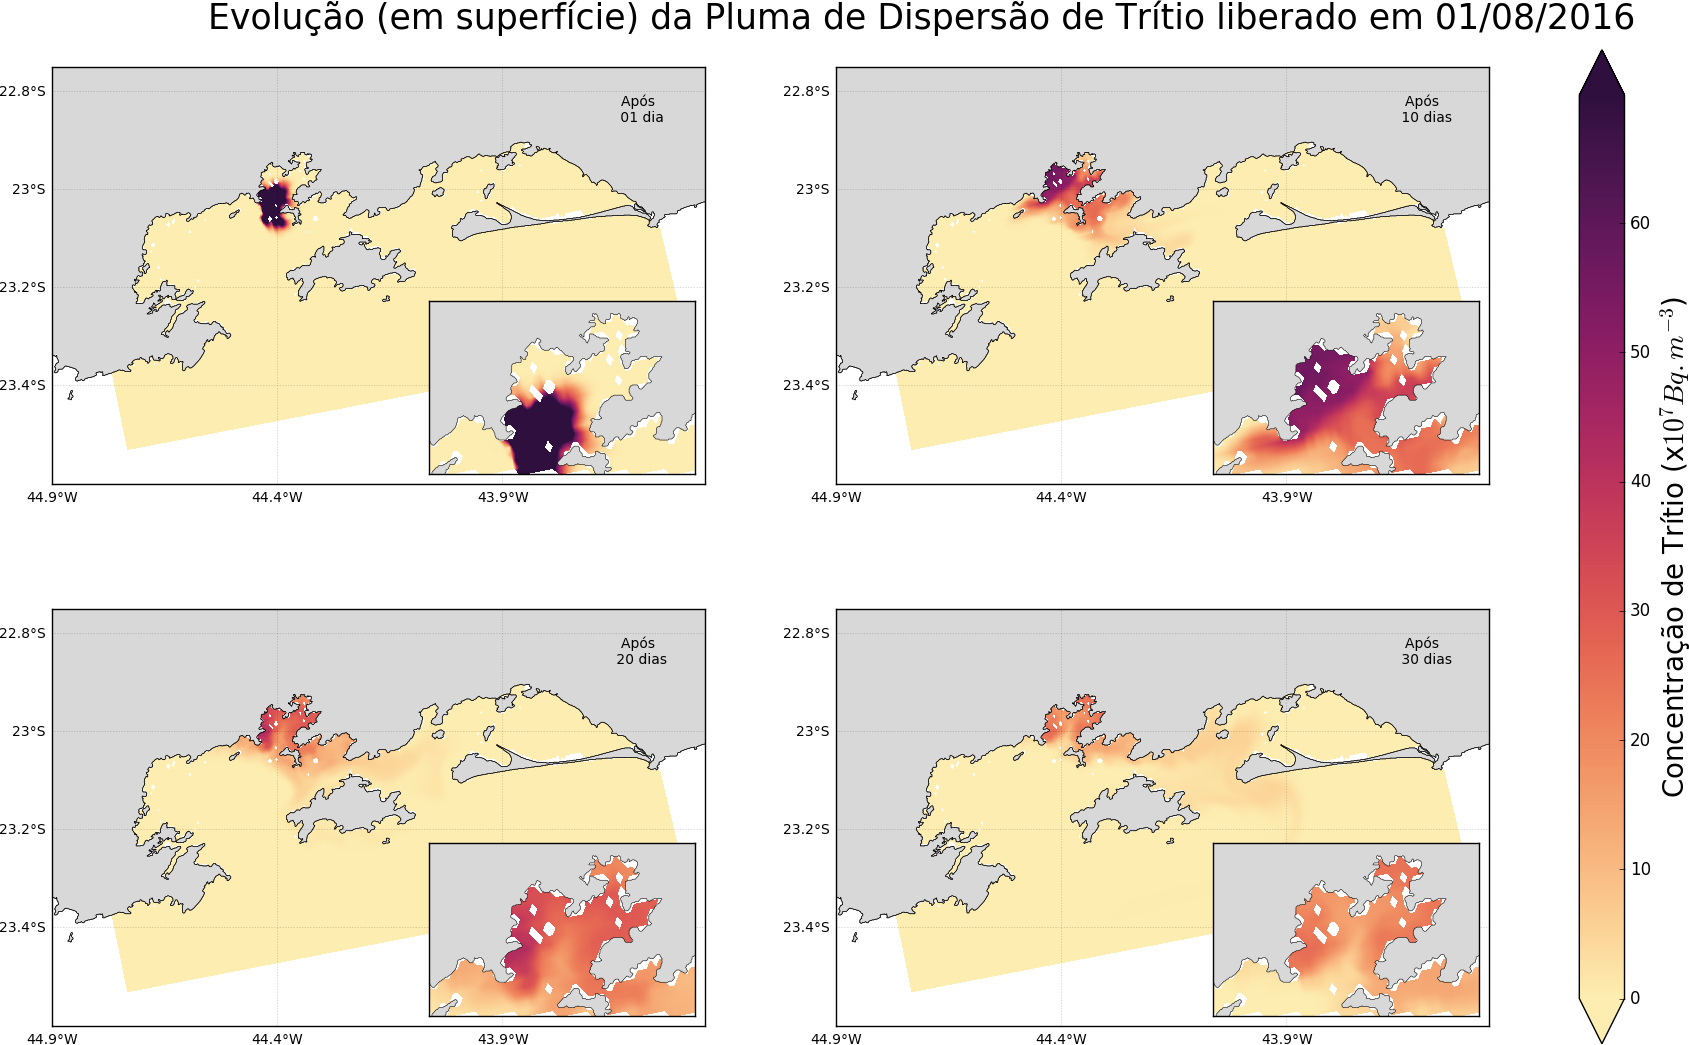
\includegraphics[width=0.9\columnwidth]{/home/tparente/danilo/mestrado/github/congressos/omarsat_2017/poster/sharelatex/figs/figura3_superficie.png}
\caption{Dispersão da pluma de material radioativo no cenário 6, os painéis representam, na ordem, os instantes de
6 horas, 10 dias, 20 e 30 dias após o vazamento.}
\label{fig:evolucaopluma}
\end{figure}
% \vskip2ex

% ===================================================================================================================
\vspace{-.5in}
\section{Conclusão}

Conclui-se que, em caso de vazamento nuclear na CNAAA, a presença do material
radioativo nas águas da região de estudo seria de, no mínimo, 60 dias, até uma redução a
níveis de concentração inferiores ao previsto na resolução no283 do CONAMA.
Além disso, as regiões de maior impacto seriam: Baía da Ribeira, ponto de descarte da
água e, dependendo do regime de ventos no instante do vazamento, a pluma poderá
alcançar regiões a oeste, como Paraty e Mambucaba, ou a leste, como Angra dos Reis,
Baía de Sepetiba e Marambaia.
Destaca-se que a pluma será melhor diluída ao atingir regiões a leste do
domínio estudado, onde a maré gera correntes mais intensas.

\end{multicols}

%==============================================================================
\end{frame}
\end{document}
